\documentclass[a4paper]{article}
\usepackage[utf8]{inputenc}
\usepackage[spanish, es-tabla, es-noshorthands]{babel}
\usepackage[table,xcdraw]{xcolor}
\usepackage[a4paper, footnotesep = 1cm, width=20cm, top=2.5cm, height=25cm, textwidth=18cm, textheight=25cm]{geometry}
%\geometry{showframe}

\usepackage{tikz}
\usepackage{amsmath}
\usepackage{amsfonts}
\usepackage{amssymb}
\usepackage{float}
\usepackage{graphicx}
\usepackage{caption}
\usepackage{subcaption}
\usepackage{multicol}
\usepackage{multirow}
\setlength{\doublerulesep}{\arrayrulewidth}
\usepackage{booktabs}
\usepackage{mathrsfs,amsmath}
\usepackage{hyperref}
\hypersetup{
    colorlinks=true,
    linkcolor=blue,
    filecolor=magenta,      
    urlcolor=blue,
    citecolor=blue,    
}

\newcommand{\quotes}[1]{``#1''}
\usepackage{array}
\newcolumntype{C}[1]{>{\centering\let\newline\\\arraybackslash\hspace{0pt}}m{#1}}
\usepackage[american]{circuitikz}
\usetikzlibrary{calc}
\usepackage{fancyhdr}
\usepackage{units} 

\graphicspath{./Imagenes}

\pagestyle{fancy}
\fancyhf{}
\lhead{22.05 ASSD}
\rhead{Mechoulam, Lambertucci, Rodriguez, Londero}
\rfoot{Página \thepage}

\begin{document}

\subsection{Sintesis por muestras}
La Síntesis por muestras tiene sus origines en los estudios de grabación. Previo a las técnicas de Síntesis
se debían grabar nuevamente aquellos sonidos que no satisfacían por completo a los músicos o a los ingenieros de sonido obligandolos a utilizar más horas el estudio de grabación
lo cual, por supuesto, llevaba varios gastos asociados y retrasaba la culminación del proyecto.

\subsubsection{Time Stretching}
Supongamos que deseamos grabar un comercial de televisión y por cuestiones legales debemos añadir una pequeñas aclaraciones al final del mismo. Sin embargo, el tiempo de aire es altamente costoso entonces tenemos que poder incluir toda la información necesaria en un espacio de tiempo muy pequeño. Entonces podríamos suponer que basta con grabar el mensaje a velocidad de habla normal y luego reproducirlo más rápido para que ocupe menos tiempo. Es decir reproducir el sonido salteándose segmentos para poder acortar la duración. 

\begin{figure}[H]
	\centering
	\begin{subfigure}[b]{0.4\linewidth}
		\centering
		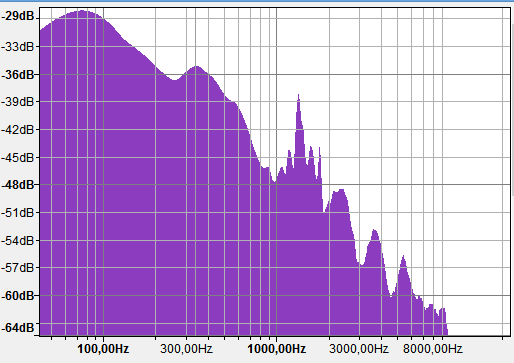
\includegraphics[scale=0.5]{ImagenesEjercicio5/HumanSpeechNormalSpeed.PNG}
		\caption{Espectro de un discurso hablado a velocidad normal}
		\label{fig:speechNormal}
	\end{subfigure}
	~
	\begin{subfigure}[b]{0.4\linewidth}
		\centering
		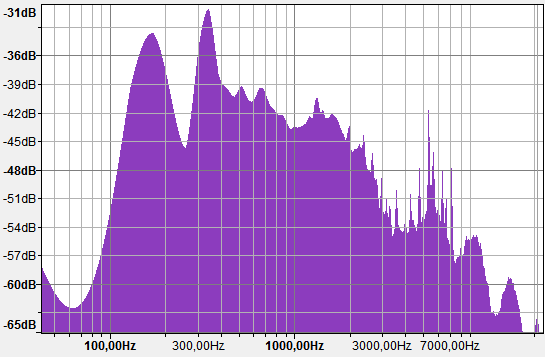
\includegraphics[scale=0.5]{ImagenesEjercicio5/HumanSpeech4X.PNG}
		\caption{Espectro del discurso con una velocidad 4 veces mayor}
		\label{fig:speech4X}
	\end{subfigure}
	\caption{Consecuencias de la compresión temporal}
\end{figure}

Como se puede observar, la figura \ref{fig:speechNormal} representa el espectro de habla de una persona hablando a una velocidad promedio. Notamos que la zona de mayor contenido armónico se halla aproximadamente entre los $80Hz$ y $200Hz$. Sin embargo, si miramos al espectro del mismo discurso pero ahora con 4 veces menos duración,figura \ref{fig:speech4X}, podemos observar que el espectro no se preservo. De hecho se puede notar que hay mayor potencia espectral a frecuencias más altas que en el espectro original. Esto se traduce en un sonido chillón que poco nos recuerda al discurso original. De forma análoga si por alguna razón se quisiera aumentar o reducir el pitch de una pista de audio se debería recurrir al método de acortar la pista o en el caso contrario alargarla. 
En la siguiente sección se explora como es posible controlar la duración y el pitch de una pista de audio de manera independiente.

\subsubsection{TD-PSOLA}
\textbf{TD-PSOLA} son las siglas para Time Domain Pitch-Synchronous Overlap-Add. 
\\
Los algoritmos basados en \textbf{PSOLA} se basan en la reutilización de pequeños segmentos llamados \textbf{short term signals} que son el resultado de aplicar una ventana de \textbf{Hanning}, que se extienda hacia los pitch-marks vecinos, sobre cada \textbf{pitch-mark} (más acerca de pitch-marks en la siguiente sección) y solaparlos convenientemente.

\begin{figure}[H]
	\centering
	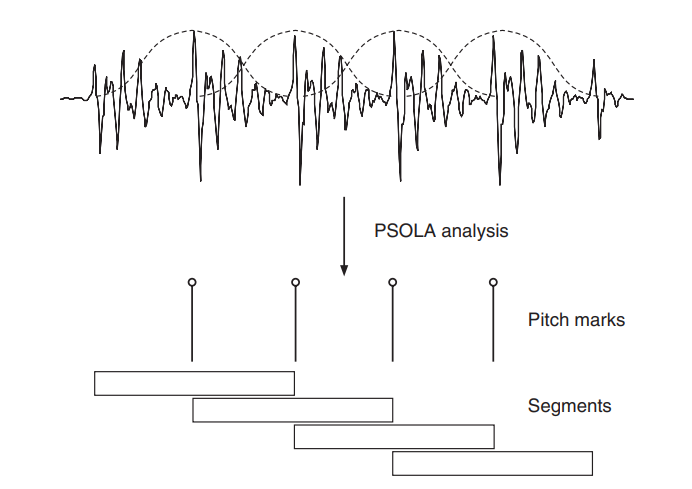
\includegraphics[width=0.7\linewidth]{ImagenesEjercicio5/PSOLA_MAIN_IDEA.PNG}
	\caption{Segmentación del sonido de acuerdo a los pitch-marks}
	\label{fig:clarification-of-the-psola-technique-adopted-from-kortekaas-1997}
\end{figure}

Para poder conseguir alargar la duración de los sonidos sin alterar así el \textbf{pitch} del mismo es necesario conservar la forma de los segmentos que la conforman.

\begin{figure}[H]
	\centering
	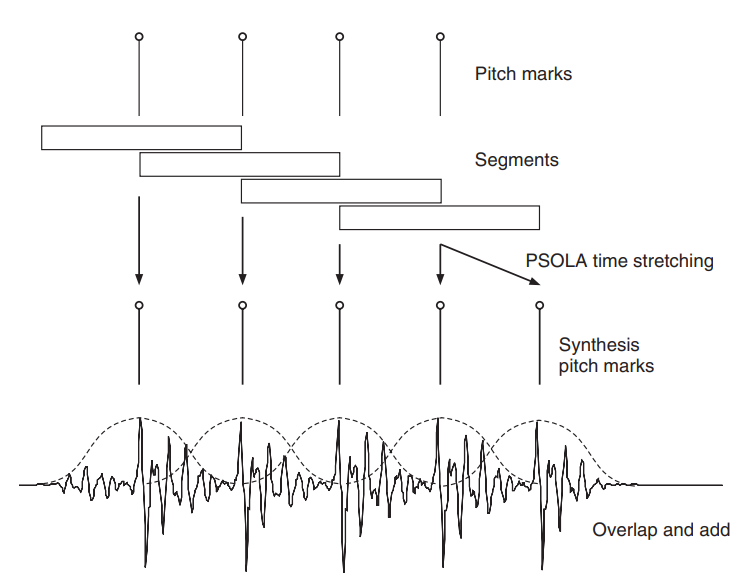
\includegraphics[width=0.7\linewidth]{ImagenesEjercicio5/TimeStretchingPSOLA.PNG}
	\caption{Ilustración del estiramiento temporal usando PSOLA}
	\label{fig:TSPSOLA}
\end{figure}

Esto se expresa dentro del algoritmo de estiramiento como un factor $\alpha = \frac{d_{nueva}}{d_{original}}$ que nos permite mapear la posición de los pitch-marks dentro de nuestro sonido original hacia el sonido de llegada. Las ventanas de Hanning son de gran utilidad porque permiten transiciones más suaves entre cada segmento.


Para poder tener control sobre el \textbf{pitch} del sonido debemos cambiar la distancia entre entre los pitch-marks para así afectar a la frecuencia fundamental $f_0$ del sonido. Análogamente, este escalado en frecuencia viene denominado como un factor $\beta = \frac{f_{nueva}}{f_{original}}$.

Estos dos factores en combinación nos permiten regular tanto el \textbf{pitch} como la duración del sonido.

\begin{figure}[H]
	\centering
	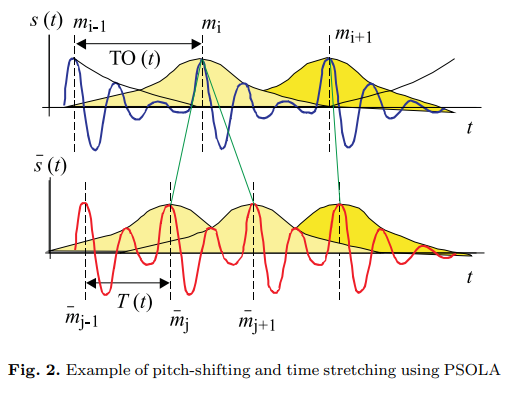
\includegraphics[width=0.7\linewidth]{ImagenesEjercicio5/PTS}
	\caption{}
	\label{fig:pts}
\end{figure}

\subsubsection{Estimación de los Pitch-Marks}
Los \textbf{pitch-marks} representan momentos del sonido en el que su amplitud es máxima en un entorno, en realidad este termino se emplea cuando se habla de \textbf{glottal pulses} dentro del campo de Voice Processing y hacen referencia a ciertos impulsos de aire genera nuestra habla.
Estas posiciones son centrales para la estructura del sonido. Poder localizarlos con precisión son un punto clave para los algoritmos que se basan en ellos para sintetizar nuevos sonidos.
\begin{figure}[H]
	\centering
	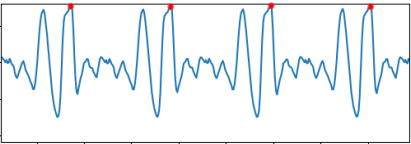
\includegraphics[width=0.7\linewidth]{ImagenesEjercicio5/soundZoomPMS.PNG}
	\caption{Imagen aumentada de una nota musical}
	\label{fig:soundzoom}
\end{figure}
En la figura \ref{fig:soundzoom} se pueden apreciar los pitch-marks estimados para la nota \textbf{A4}. En este caso podemos decir, mediante inspección visual, que se la estimación ha tenido un éxito considerable. Sin embargo, estimarlos para una sonido más complejo como puede ser la voz humana o una pista de audio no es una tarea sencilla y se deben tener en cuenta varios factores.
Para la estimación de los pitch-marks de las notas se utilizo el programa \textit{Audacity} para visualizar el espectro y obtener la frecuencia fundamental de la nota $f_0 = 395Hz$. A partir de la frecuencia fundamental y el previo conocimiento del \textbf{sample rate} de la muestra se realizaran las siguientes hipótesis.
	
	$$	P \approx 1/f_0 = 2.53ms$$
Es decir que $P$, el \textbf{pitch-period}(tiempo entre pitch-marks) tendrá aproximadamente esa duración.
$$ M_p = \frac{sampling\;rate}{f_0} = \frac{44100}{395} \approx 112\; muestras  $$
Este dato nos indica que entre cada pitch-mark tenemos 112 puntos de espacio. Con este dato es posible utilizar el paquete científico \textit{Scipy} y calcular los máximos de la señal que estén equiespaciados por lo menos 112 muestras entre sí.
\begin{figure}[H]
	\centering
	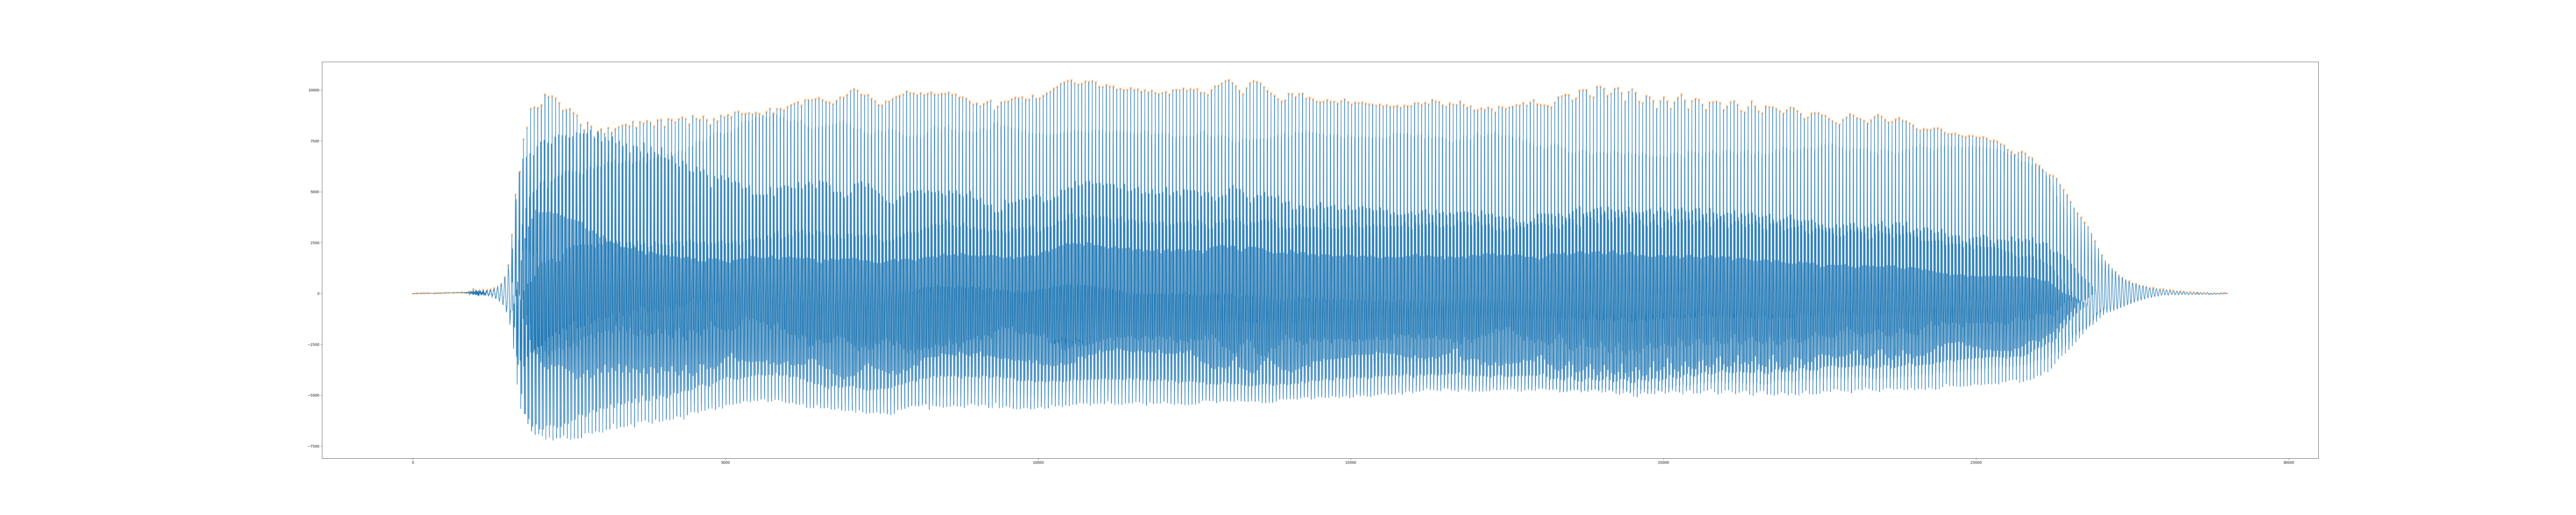
\includegraphics[width=\linewidth,height=150px]{ImagenesEjercicio5/noteA4}
	\caption{Pitch Marks en una Nota A4 de Saxofón, $f_0$ = $395Hz$ (poner el zoom  al maximo y mirar en la parte superior)}
	\label{fig:pmsnotea4}
\end{figure}

Como se puede apreciar en la figura \ref{pmsnotea4} este método funciona bien para la nota A4. Sin embargo al probar este método sobre la nota $A\#6$

\begin{figure}[H]
	\centering
	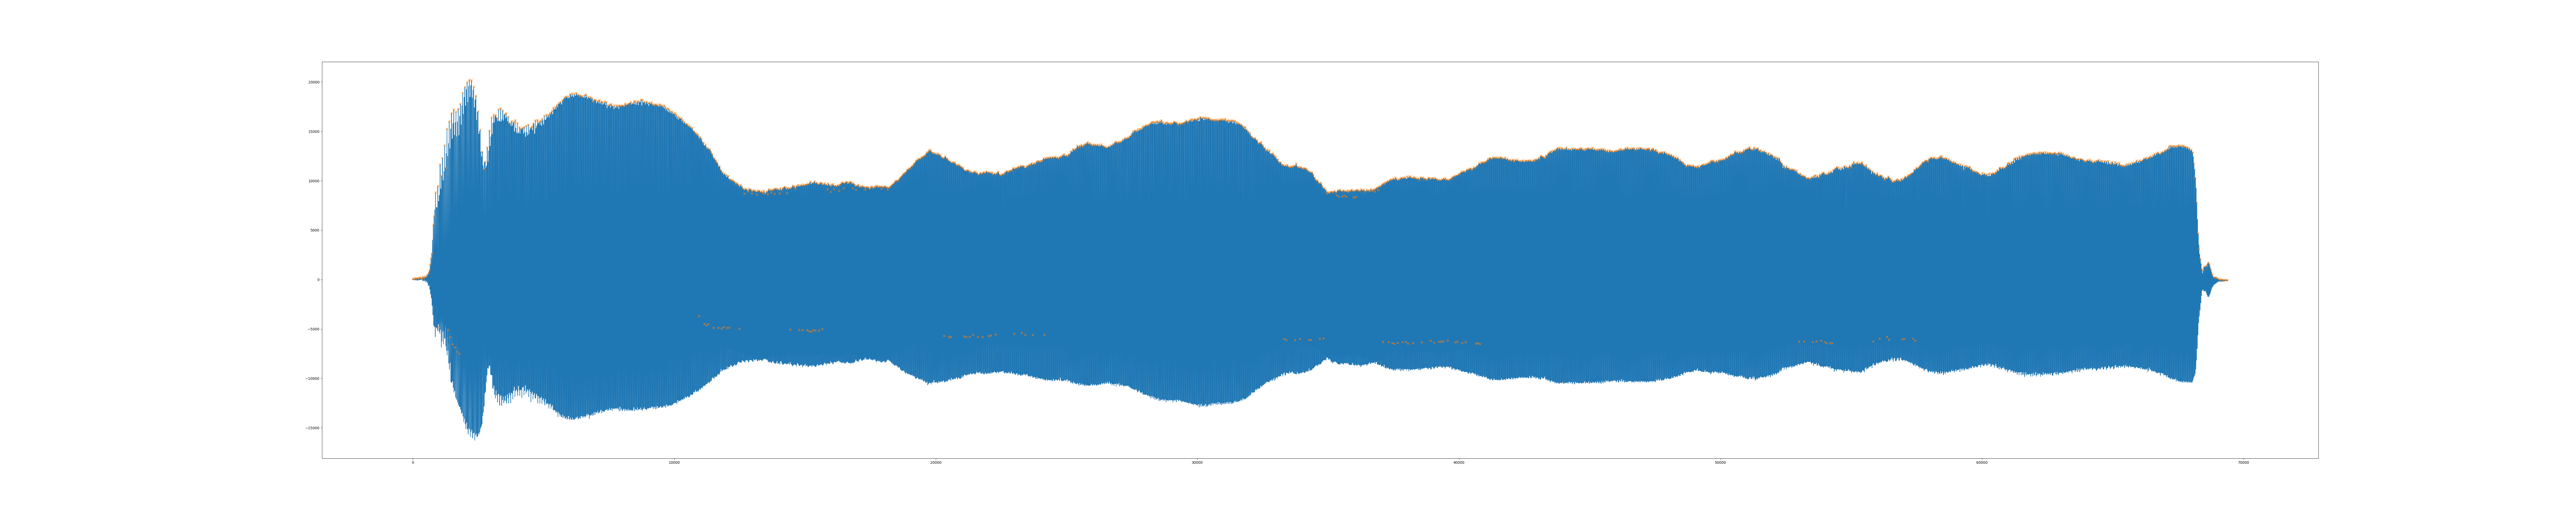
\includegraphics[width=\linewidth,height=150px]{ImagenesEjercicio5/Asharp6.png}
	\caption{Pitch Marks en una Nota A6 de Saxofón(poner el zoom  al maximo y mirar en la parte superior)}
	\label{fig:pmsnotea4}
\end{figure}
no se obtiene resultados óptimos.






 











\end{document}